%\documentclass[12pt]{article}
%\usepackage{ctex} % 中文支持
%\usepackage{titling} % 标题格式定制
%\usepackage{lipsum} % 示例文本
%\usepackage{titlesec} % 标题格式定制
%\usepackage{graphicx}
%
%% 设置标题格式
%\titleformat{\section}{\centering\Large\bfseries}{\thesection}{1em}{}
%\titleformat{\subsection}{\centering\large\bfseries}{\thesubsection}{1em}{}
%\titleformat{\subsubsection}{\centering\normalsize\bfseries}{\thesubsubsection}{1em}{}
%
%% 调整标题位置
%\setlength{\droptitle}{-4cm}

\documentclass[UTF8]{ctexart}
\usepackage{lmodern}
\usepackage{amsmath}
\usepackage{amssymb}
\usepackage{graphicx}
\usepackage{geometry}
\usepackage{xcolor}

\geometry{left=2.18cm,right=2.18cm,top=1.54cm,bottom=2.0cm}
\pagestyle{empty}
\title{\bf 2025秋计算方法--实验报告 \#2---16分(含编程小结2分)}
\author{姓名：金天昊 \quad 学号：PB24000144 }
\date{\today}

\begin{document}

%\title{\huge{\textbf{2023秋计算方法-实验报告\#1}}}
%\author{姓名：\underline{   }\hspace{1cm}学号：PB2151xxxx}
\maketitle
运行环境：Windows 11，VSCode，MSVC 19.42.34436（实验程序）

运行环境：Windows 11，VSCode，CPython 3.13.6（画图程序）
%win11，vscode，py3

\section*{实验内容与要求}
分别编写~Newton 迭代法 (通常也称 Newton-Raphson 迭代法)
$$\color{blue} x_{n+1}=x_n-\frac{f(x_n)}{f'(x_n)}$$
和 %Damped-Newton (DN) 迭代
%霍氏迭代法
Steffensen 迭代法
%\begin{center}
%\end{center}
   % $x_{k+1}=x_K-\tau\frac{f(x_k)}{f'(x_k)}$，(其中阻尼参数$\tau$: 0 <$\tau$< 1)
 %$$\color{blue}  x_{n+1}= x_n - \frac{2f(x_n)f'(x_n)}{2f'(x_n)f'(x_n) - f(x_n)f''(x_n)}, \, n=0,1,2,\cdots$$
 $$\color{blue}  x_{n+1}= x_n - \frac{f(x_n)f(x_n)}{f(x_n + f(x_n)) - f(x_n)}, \,\; n=0,1,2,\cdots$$

的通用程序, 并利用它们对如下非线性方程
$$\color{blue}  f(x)\triangleq{arctan(x)}+ 0.4x \sin(\frac{x}{2}) + 0.601958 =0$$
求区间[-80,80]上的根. %取阻尼参数$\tau$=0.55,
计算中的停止条件为~$\color{red}|f(x_n)|<\varepsilon = 10^{-8}$~或迭代步数~$\color{red} n>10^4$~(可视为迭代失败).
%%提示：编程前分别手算出$\color{blue}~f'(x), f''(x)$。

\begin{itemize}
    \item 列表给出两种迭代方法在初始点 $x_0$ 依次取值~-80,-70, -55, -36, -20, -5, -3.14, -1, 0, 1.1958, 3.14, 5, 10, 22, 33, 44, 51, 60, 80~时的迭代步数
    （若迭代步数超过1万步, 或数值解超出区间[-80,80], 可视为求解失败）
    以及相应的数值解~$x_n$~(保留小数点后6位; 迭代失败时无需给出)；
    \item 比较并分析两种方法的优劣, 给出合理的算法分析并作实验小结。
\end{itemize}
\clearpage
\section{数值结果（列表或作图）}
函数~$f(x)$~图像参见图1; 计算结果参见表1.

\begin{figure}[htb]
	\centering
	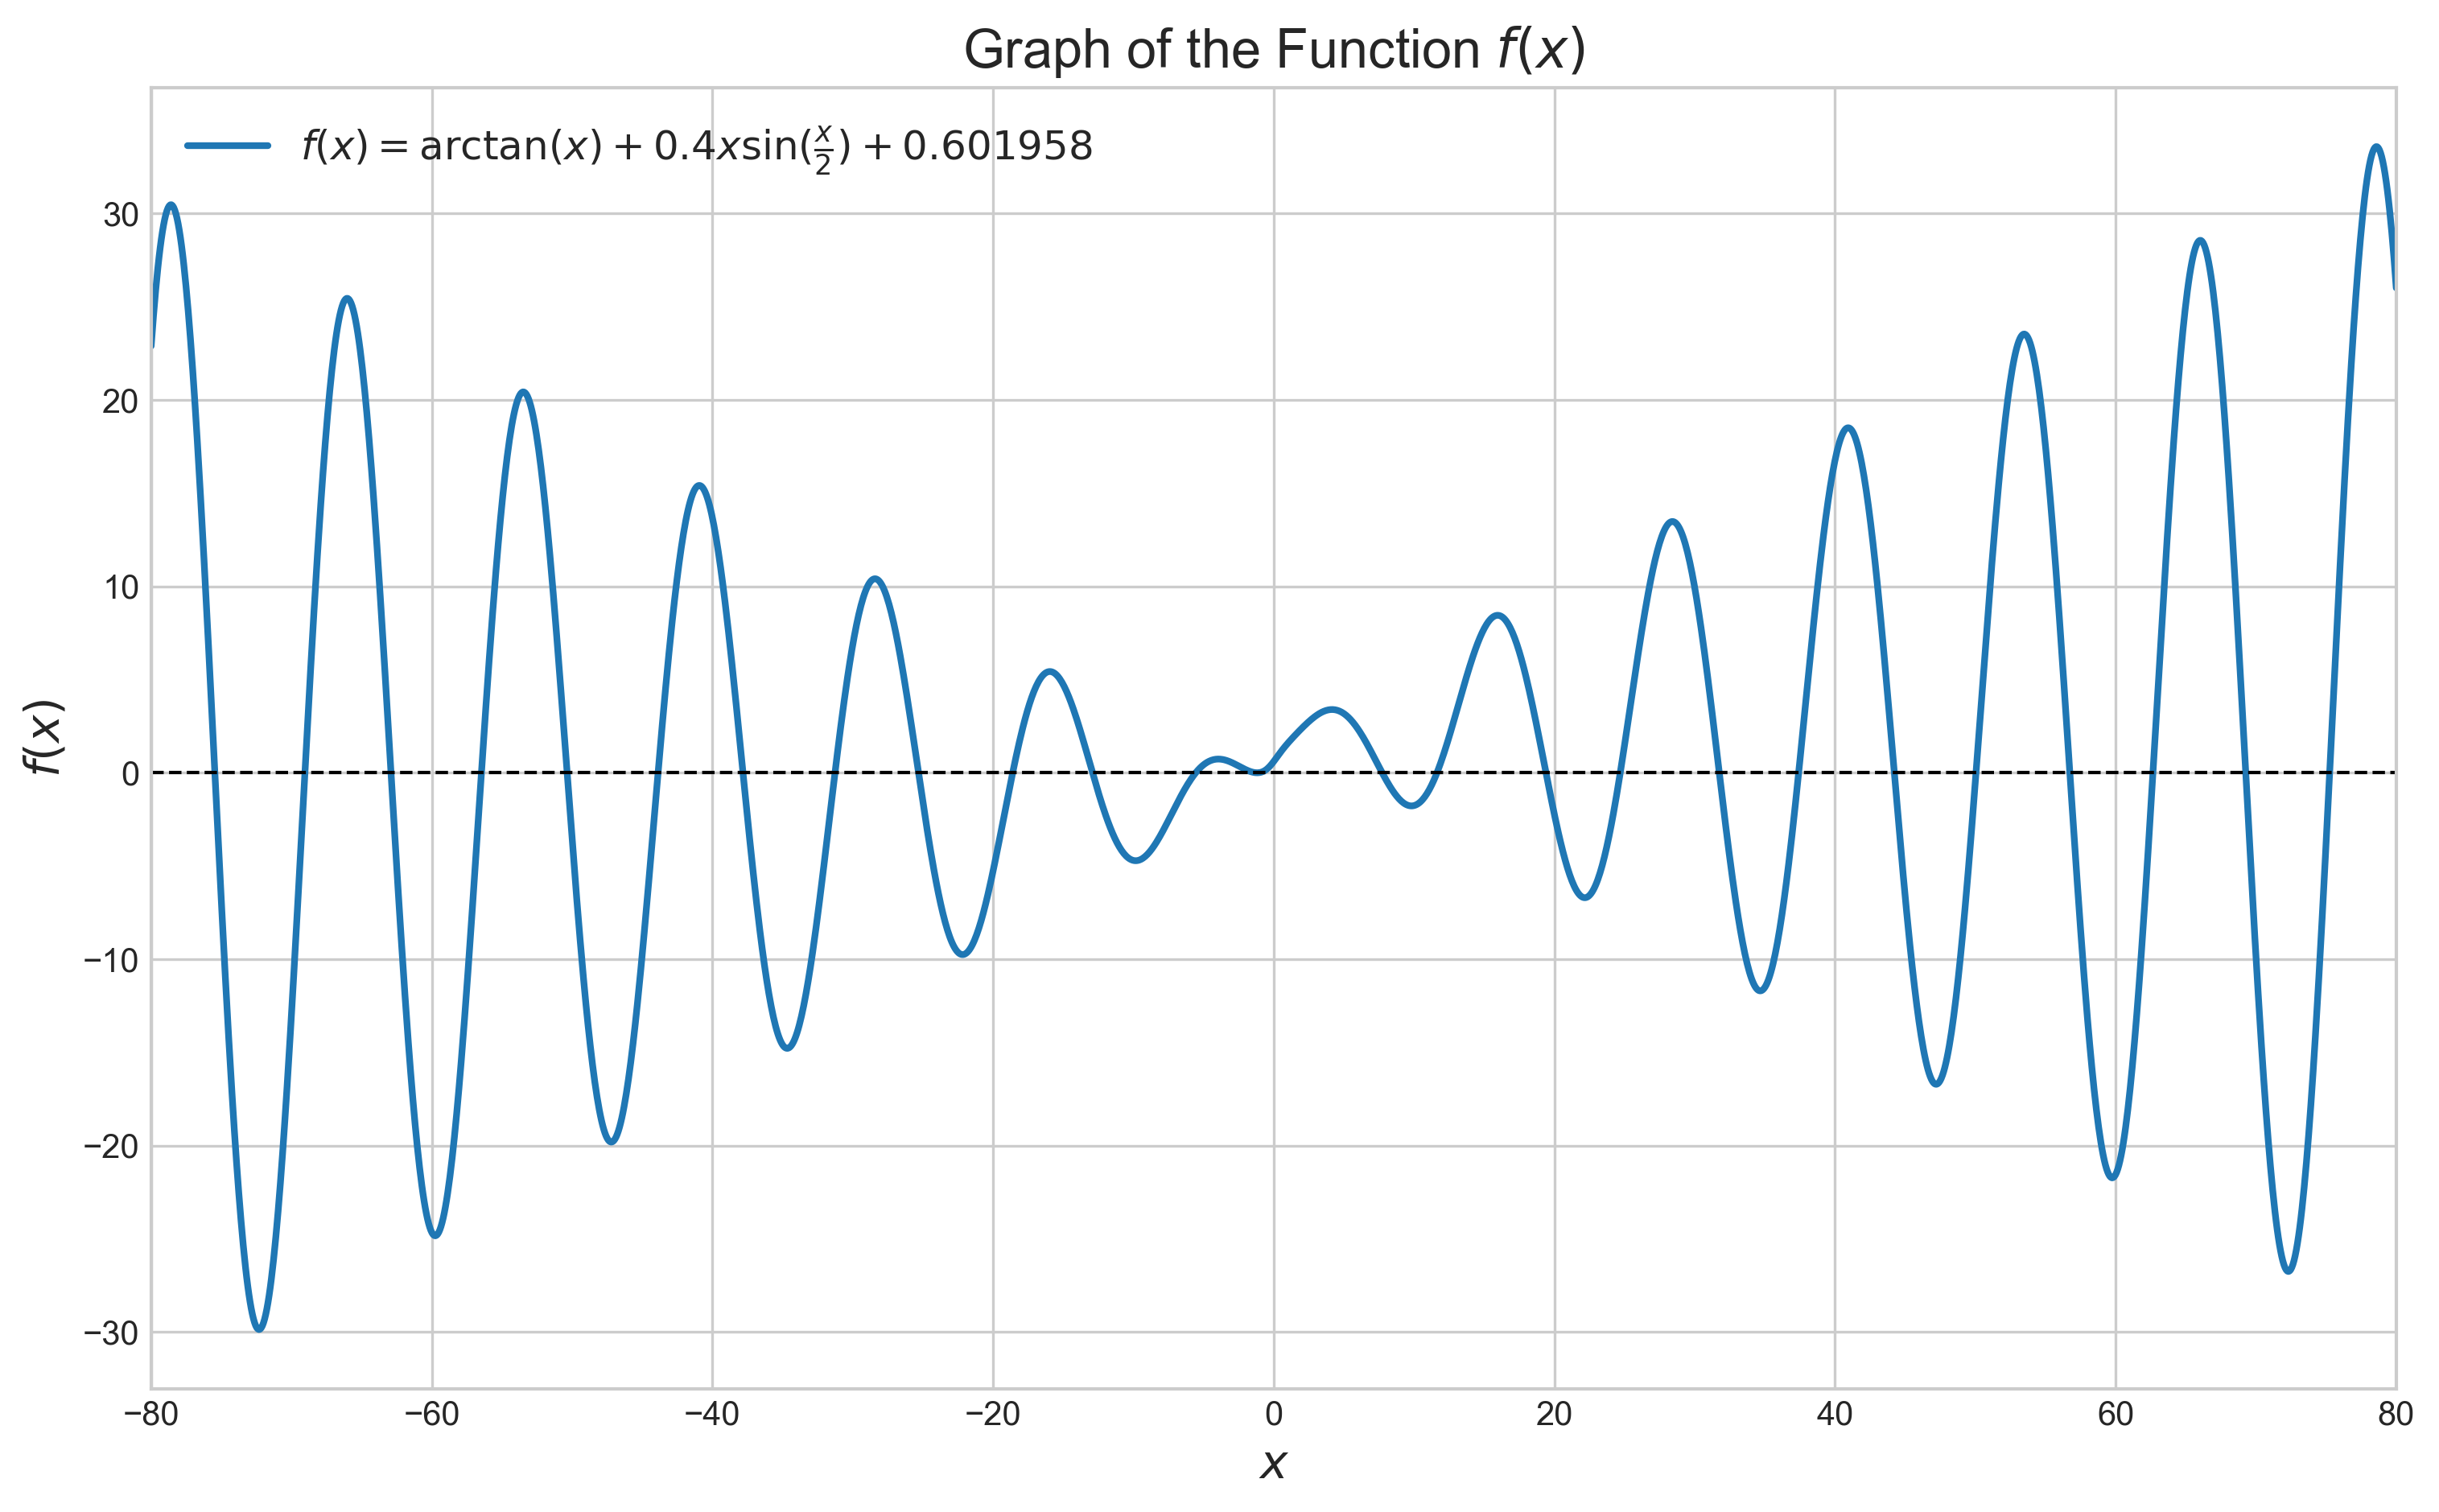
\includegraphics[width=0.4\textwidth]{f_x_graph.png}
	\caption{函数 $f(x)=\arctan(x)+0.4x\sin(\frac{x}{2})+0.601958$ 在区间 $[-80,80]$ 的图像}
	\label{fig:fx_plot}
\end{figure}

\begin{table}[htb]
\centering
\caption{计算结果: 精度~$\color{red}\varepsilon = 10^{-8}$, 最大迭代步数~$10^4$}
\begin{tabular}{cccccc}
\hline
初始点~$x_0$ & Newton法步数 & Newton法数值解 & Steffensen法步数 & Steffensen法数值解 \\
\hline
-80 & 求解失败 &  & 5 & -62.907613 \\
-70 & 3 & -69.045914 & 11 & -18.602967 \\
-55 & 4 & -56.464419 & 求解失败 &  \\
-36 & 4 & -37.823771 & 5 & -12.913315 \\
-20 & 4 & -18.602967 & 4 & -25.316548 \\
-5 & 4 & -5.555571 & 5 & -5.555571 \\
-3.14 & 6 & -1.278007 & 6 & -1.278007 \\
-1 & 4 & -1.083224 & 4 & -1.083224 \\
0 & 7 & -1.083224 & 7 & -1.083224 \\
1.1958 & 6 & -1.083224 & 6 & -1.278007 \\
3.14 & 6 & -1.083224 & 5 & 11.636464 \\
5 & 5 & 11.636464 & 3 & 7.728136 \\
10 & 4 & 19.403227 & 4 & 7.728136 \\
22 & 5 & 31.754703 & 4 & 19.403227 \\
33 & 4 & 31.754703 & 6 & -37.823771 \\
44 & 3 & 44.225986 & 3 & 44.225986 \\
51 & 3 & 50.050003 & 23 & -62.907613 \\
60 & 4 & 75.254623 & 4 & 44.225986 \\
80 & 求解失败 &  & 求解失败 &  \\
\hline
\end{tabular}
\end{table}

{\bf 对于求解失败，均是数值解超过了区间~$[-80,80]$。对于~$x_0=51$，Steffensen迭代法在超出区间后又迭代回区间并成功求解。}

\section{算法分析}
本题要求实现 Newton 迭代法和 Steffensen 迭代法的通用程序。为此，将 $f(x)$ 和其导函数 $f'(x)$ 作为已定义函数，在两种方法中作为黑盒调用。根据题目中的公式，分别实现了两个迭代法的计算，并将初始点、精度要求和最大迭代步数作为参数传入函数。主函数中依次对题目要求的各初始点调用两种方法并输出结果。

实验发现，Newton 法和 Steffensen 法对初始点的敏感性和收敛速度均较接近，且都具有极快的二阶收敛速度。不过，Newton 法需要手动计算 $f'(x)$，当导函数难以求解时不易使用；而 Steffensen 法通过 $\frac{f(x_n + f(x_n)) - f(x_n)}{f(x_n)}$ 近似替代 $f'(x_n)$，避免了求导的麻烦，但需要多计算一次 $f(x)$，在某些情况下计算量会高于 Newton 法。

%从表1中，不难观察到
% \begin{itemize}
%     \item Blah blah blah
%     \item Blah blah blah
%     \item Blah blah blah
% \end{itemize}

%Blah blah blah

%\begin{table}[H]
%\centering
%\caption{收敛范围}
%\begin{tabular}{|c|c|c|}
%\hline
%列1 & 列2 & 列3 \\
%\hline
%初始点 & Newton & Damped-Newton\\
%0 & [-0.7, 1.7] & [-1.2, 1.8]\\
%\hline
%\end{tabular}
%\end{table}
%

\section{实验小结}
在本次数值实验中，我们分别测试了两种非线性方程求根的计算方法，发现了两种算法都表现出了二次收敛的特性，能够用很少的迭代步数快速地找到高精度的数值解，在适用条件上存在显著差异，同时体会了数值算法的选择和初始值的选取对于求解成功与否的至关重要性。最终得到以下结论：

%算法的选择的重要性。最终得到以下结果：
Newton~迭代法\\
优点：在初始点选取合适且导数性质良好的情况下，算法具有二次收敛性，收敛速度极快，迭代步数少。 \\
缺点: 必须能够求解并编程实现函数的导数，适用范围受限；对初始点~$x_0$~的选取十分敏感，不好的初始点可能导致迭代因导数趋于零而发散失败。

Steffensen~迭代法\\
优点：无需计算导数，仅需调用函数本身~$f(x)$~，适用性更广，且收敛速度与牛顿法同阶，鲁棒性更强。 \\
缺点: 每次迭代需要进行两次函数值的计算，如果函数~$f(x)$~本身的计算非常耗时，那么其单步计算成本可能会高于 Newton 法。



\end{document}
